\documentclass[12pt]{article}
\usepackage{a4wide}
\usepackage{anysize}
\usepackage{latexsym}
\usepackage{algorithmic}
\usepackage{amssymb}
\usepackage{epsfig}
%\usepackage{psfig}
%\usepackage{tabls}
\usepackage{multicol}
\usepackage[dvips]{color}
\usepackage{booktabs}% http://ctan.org/pkg/booktabs
\usepackage{float}
\usepackage{tabularx}
\usepackage[section]{placeins}
\usepackage{graphics}
\usepackage{array}
\usepackage{longtable}
\usepackage{supertabular}
\usepackage{tabularx}
\usepackage{ltablex}
\newcolumntype{L}{>{\centering\arraybackslash}m{3cm}}



\usepackage{graphicx} 
%\usepackage[pdftex]{graphicx}
\setboolean{@twoside}{false}


%\usepackage[T1]{fontenc}

\newcommand{\tabitem}{~~\llap{\textbullet}~~}
\marginsize{1.5cm}{1.5cm}{1.5cm}{1.5cm}
\def\baselinestretch{1}                          
\begin{document}
%\baselineskip 20pt
%The definitions
\def\title{Gamification of Video Classification}
\def\what{M. Tech. Project Stage 1 Report}
\def\degree{Master~of~Technology}
\def\who{V Sai Saketh Ram}
\def\roll{13305R010}
\def\guide{Prof. Ganesh Ramakrishnan}
% \titlpage
\begin{center}
\vspace{0pt plus 2fil}
{\LARGE \bf \title}\\ 
\vspace{0pt plus 0.7fil}  
{\bf \what}\\
\vspace{0pt plus 0.3fil}
Submitted in partial fulfillment of the requirements\\
for the degree of\\
\vspace{0pt plus 0.2fil}
{\bf \degree}\\
\vspace{0pt plus 0.5fil}
by\\ 
\vspace{0pt plus 0.2fil}
{\bf \who}\\
\vspace{0pt plus 0.05fil}
{\bf Roll No: \roll} \\
\vspace{0pt plus 0.5fil}
under the guidance of\\
\vspace{0pt plus 0.2fil}
{\bf \guide}\\
\vspace{0pt plus 2fil}





\begin{figure}[h]
\begin{center}
 



\includegraphics{images/iitblogo.jpg}
\end{center}
\end{figure}





\vspace{0pt plus 2fil}
Department of Computer Science and Engineering \\ 
Indian Institute of Technology, Bombay \\ 
Mumbai\\
\vspace{0pt plus 1fil}
\today \\
\end{center}
\def\bsq{\begin{flushright} $\blacksquare$\\ \end{flushright}}
\def\tab{\hspace{5mm}}
\newpage
%The stuff



\pagenumbering{roman}
\begingroup\def\thispagestyle#1{}\def\baselinestretch{1.5}\tableofcontents\endgroup     
\newpage
%% -*- LaTeX -*-

\begin{abstract}
The main objective is to optimize the game called "tagVideo", a Game With A Purpose(GWAP) that collects tags of videos to better
understand videos and how people go about tagging.When people play the game they help determine the contents of videos
by providing meaningful labels for them.Rather
than using computer vision techniques to get the categories for videos, which don’t work
well enough, we encourage people to do the work by taking
advantage of their desire to be entertained.

The major application of tagVideo game is that collected tags can help provide more effective searches, intuitive navigation, and data for
training video classification models.



\end{abstract}

\newpage
\pagenumbering{arabic}

%\newpage
%\section{Introduction}

\subsection{Background} 
Researchers have many software options to write papers,But fewer to collaborate with others.
Two main Reasons for less use of versioning systems are Usability problems and Need for users to resolve conflicts.
We will compare google docs with other solutions. And also extensions to google docs to overcome its drawbacks.

\subsection{Existing solutions}
Current existing solutions for collaborative editing are-
\begin{itemize}
 \item E mail
 \item CVS and SVN

 \end{itemize}
 
 \subsubsection{E mail}
 \begin{itemize}
  \item  purely sequential
 \item  conceptually simple
 \item  others cannot contribute
 \item  sent to a single collator
 \end{itemize}
 
 \subsubsection{CVS and SVN}
 \begin{itemize}
 \item single server maintains repository
\item check out,check in concepts
\item user must have client software installed
\item resolving conflicts
\item only text based files
 \end{itemize}
 
 
 
 
 
 


\subsection{Reasons for still using older Techniques}
\begin{itemize}
\item Usability,update and commit concepts
\item user accounts have to be managed
\item need to resolve conflicts
\end{itemize}

\subsection{Google Docs}
\begin{itemize}
 
 \item  Author edits a doc on google repository.
 \item  uses simple browser editor developed by AJAX
 \item  There is also viewer category
 \item  Changes to docs are automatically transmitted to server(every 30 seconds)
 \item  Because of high frequency of updates,conflicts are unlikely
 \item  Doc can be saved in various formats like PDF,HTML
\end{itemize}


\subsection{Shortcomings of Google Docs}\cite{2006}


\begin{itemize}
  \item Editor problems
 \item Academic requirements
 \item Offline support
 \item Docs reside on google server.So no gaurantee of security
 \item Text based only
 \item Hard to control output layout
 \item Vendor independence(cannot use favorite editors)
\end{itemize}



\subsection{Extending Google Docs}\cite{2006}
\begin{itemize}
   \item Automatic conversion to LATEX
  \begin{itemize}
   
  \item Importing google docs
  \item Initial cleansing
  \item Canonicalization
  \item Latex transformation
  \item Security issues
   \end{itemize}

  \item Synchronizing offline documents
\end{itemize}





%The report is organized as follows: Section 1 provides the background knowledge and the need for a continuous authentication model for smart phones.
%Section 2 discusses about general experiment setup.
%Section 3 discusses about the various approaches and their performance in authentication. Future scope is discussed in section 5. 
%Section 6 draws the conclusions for the work done.

\newpage
\section{Introduction}
There are large number of video collection and they present major technological challenge to classify them. There are no proper guide lines to provide textual description for videos,   but yet this information is very much essential for major applications like video search engines.To make this manul process more enjoyable we introduce a game with a purpose(GWAP) called \textbf{"tagVideo"} .

\subsection{tagVideo game}
tagVideo is a game that lets you tag interesting videos. You can also view these videos on YouTube to gain knowledge.And for the tags entered, player can see the scores for each tag which motivates him/her to give more related tags.

\begin{figure}[h]
\begin{center}
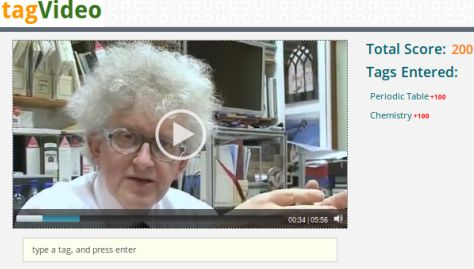
\includegraphics{images/gamedashboard.jpg}
\caption{tagVideo game}
\label{agree on image}
\end{center}
\end{figure}

\newpage
After the player finishes the game, he/she will be shown the leaderboard where rankings of all the players are displayed.This can be seen in Figure ~\ref{leaderboard}

\begin{figure}[h]
\begin{center}
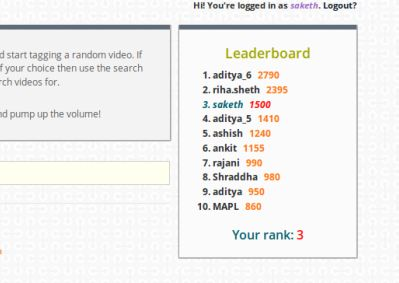
\includegraphics{images/leaderboard.jpg}
\caption{Leaderboard displaying scores}
\label{leaderboard}
\end{center}
\end{figure}


\newpage
\section{Related Work}
\subsection{ESP Game\cite{esp}}
\textbf{ESP}(Extra Sensory Perception) game is a similar game that allows users to tag images. This game is played by 2 partners and meant to be played online by large number of pairs at once. Partners are randomly assigned and do not know each other. The only thing they have in common is the image that they tag. 

\textbf{Goal :}\\
From the player's perspective the goal of the ESP game is to guess what their partner is typing. Once they type the same string, then they move on to next image. They need not enter the tag at same time, but each must type the same string at some point while the image is on the screen.Please see Figure ~\ref{agree on image} for understanding this scenario. \\

\begin{figure}[h]
\begin{center}
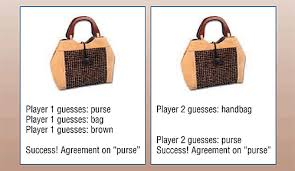
\includegraphics{images/esp_handbag.jpeg}
\caption{partners agreeing on an image}
\label{agree on image}
\end{center}
\end{figure}

\textbf{Taboo} words are the words that the player is not allowed to enter as guesses. Initially an image will have no taboo words.When it is used for second time, it will have one taboo word obtained from agreement on that image from previous game and so on.Please see Figure ~\ref{taboo words} that displays taboo words of ESP game.\\ \\
The rationale behind these taboo words is that often
the initial labels agreed upon for an image are the most
general ones (like “man” or “picture”), and by ruling those
out the players will enter guesses that are more specific.
Additionally, taboo words guarantee that each image will
get many different labels associated with it.\\ \\ \\ \\ \\ \\ \\ \\ \\


\begin{figure}[htb]
\begin{center}
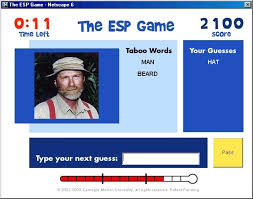
\includegraphics{images/esp_thermometer.jpeg}
\caption{Thermometer measures number of images agreed}
\label{taboo words}
\end{center}
\end{figure}

The differences between current existing ESP game and our tagVideo game is depicted in the following table. \\






 \begin{table}[htb]
	\begin{center}
	 
 
\begin{tabular}{||c||c||} 

\hline
 \textbf{ESP game} & \textbf{tagVideo game} \\ [0.5ex] 
 \hline\hline
 Tags Images & Tags Videos \\ 
 \hline
 
 Atleast two players must be online at the same time & No restriction  \\
 \hline
 
  Single game is for 2.5 minutes & No restriction on time  \\
 \hline
 
   Score is given only for common entered tag & Score is given for all tags(if related to video)  \\
 \hline
 
 \end{tabular}
 \caption{Comparison of ESP and tagVideo games}
 \end{center}
 
\end{table}





\newpage
\section{IBM Watson services used in the game}
\subsection{Concept Insights\cite{conceptinsights}}
\textbf{Concept Insights} service is used to explore information based on the concepts in the input, rather than limiting finding to traditional text matching. For example, if we search by entering the input as \textbf{\textit{disaster}}, then the concept insights service not only gives the output that contains the word "disaster" but also terms like \textbf{\textit{Earthquake}}, \textbf{\textit{Drought and Famine}}, \textbf{\textit{Hurricane}} and so on.\\


\textbf{API Overview :}\\
Concepts Insights service consists of 3 inter-connected end points.
\begin{itemize}
\item Accounts end point
\item Graph end point
\item Corpora end point
\end{itemize} 

\subsubsection{Accounts end point}
This allows user to retrieve concept insights identification information.This information can be used from other APIs to allow users to create and name their own resources.

\subsubsection{Graph end point}

This is the main end point whose functions are used in the tagVideo game.This allows user to navigate and explore concept insights knowledge graph.
The functions of this end point that are used in the tagVideo game are:
\begin{enumerate}


\item{\textbf{label\_search }}\\
Searches concepts in a concept graph looking for partial matches on the concept label field. The comparison is not case sensitive. When the prefix parameter is set to true, the main use of this method is to build query boxes that offer auto-complete, to allow users to select valid concepts.

\textbf{Input parameters}
\begin{itemize}


\item Text that indicates concept to be searched for. 
\item prefix if set to true, works as auto complete feature.
\item limit, that indicates number of suggestions to be shown in ouput.(In game, it is set to 6)
\end{itemize}
\textbf{Output parameters}
\begin{itemize}


\item JSON Array of different senses that are related to input concept.

    \end{itemize}
    
  \textbf{Example}\\
  
  Input : scie
  
  Output: 
  
  1. Science\\
  2. Science \& Technology center\\
  3. Science \& religion\\
  4. Science \& technology in Israel\\
  5. Science \& Faith tour\\
  6. Science \& technology\\
  
  This can be depicted in the Figure ~\ref{auto suggestions}.\\
  
  
\begin{figure}
\centering
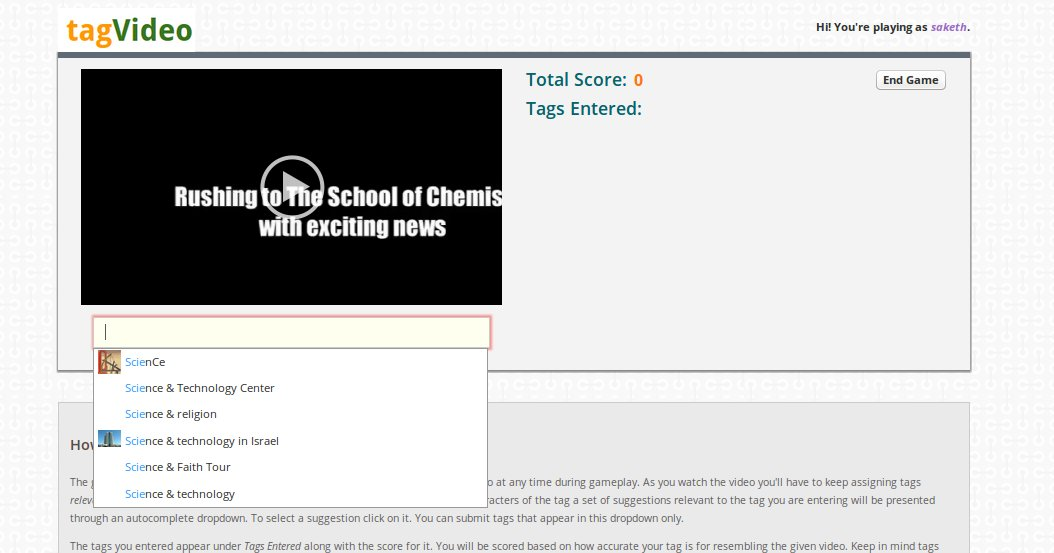
\includegraphics[width=520pt,height=300pt,scale=0.8]{images/auto_sug.jpg}
\caption{Label\_search function used with prefix set to true}
\label{auto suggestions}



\end{figure}
  
  
  

\textbf{Where it is used in the game?}\\
This function is used in 2 places in the tagVideo game.

1) While searching for videos that has to be selected to start playing the game with.\\
2) While entering the tags,to get auto suggestions on fly for the entered tag.\\
\item{\textbf{related\_concepts }}\\
Retrieve concepts that are related (in conceptual sense) to a given concept or set of concepts. The method returns an array of Concepts. Each entry is augmented with a score field, which is a probability (value between 0.5 and 1.0) of the query concept being related to the concept in the returned entry.






\textbf{Input parameters}
\begin{itemize}


\item Array of concepts. 
\item  level parameter.

The level parameter is an important option for this method. It allows the caller to choose the level of abstraction (or popularity) of the returned concepts. Values of 0 indicate very popular concepts (sometimes, they are also high level) concepts, such as countries, institutions, celebrities and subject areas. Values of 1-3 indicate increasingly less well known concepts that are likely to be related to fewer and fewer other concepts, and are more domain-specific concepts.

\end{itemize}
\textbf{Output parameters}
\begin{itemize}


\item JSON Array of suggested concepts

    \end{itemize}
    
  \textbf{Example}\\


Input: Farming,Irrigation,Food,Crops\\

Output:\\

 \emph{Level 0}: Irrigation,Food,Agriculture,Soil,Groundwater\\
 \emph{Level 1}:Sustainable agriculture,Food security,List of sustainable agriculture topics,
Index of soil related articles,Tillage,Soil science,Permaculture\\
\emph{Level 2}:International water management institute\\
Good agricultural practices\\
Environmental impact of agriculture\\
Agricultural productivity\\








 

  

\textbf{Where it is used in the game?}\\
Right now this function is not used in the game.  But as a future extension, This has to be used 

1) To suggest additional tags to the player based on the tags he had already entered.
\end{enumerate}



\begin{figure}
 \centering 
 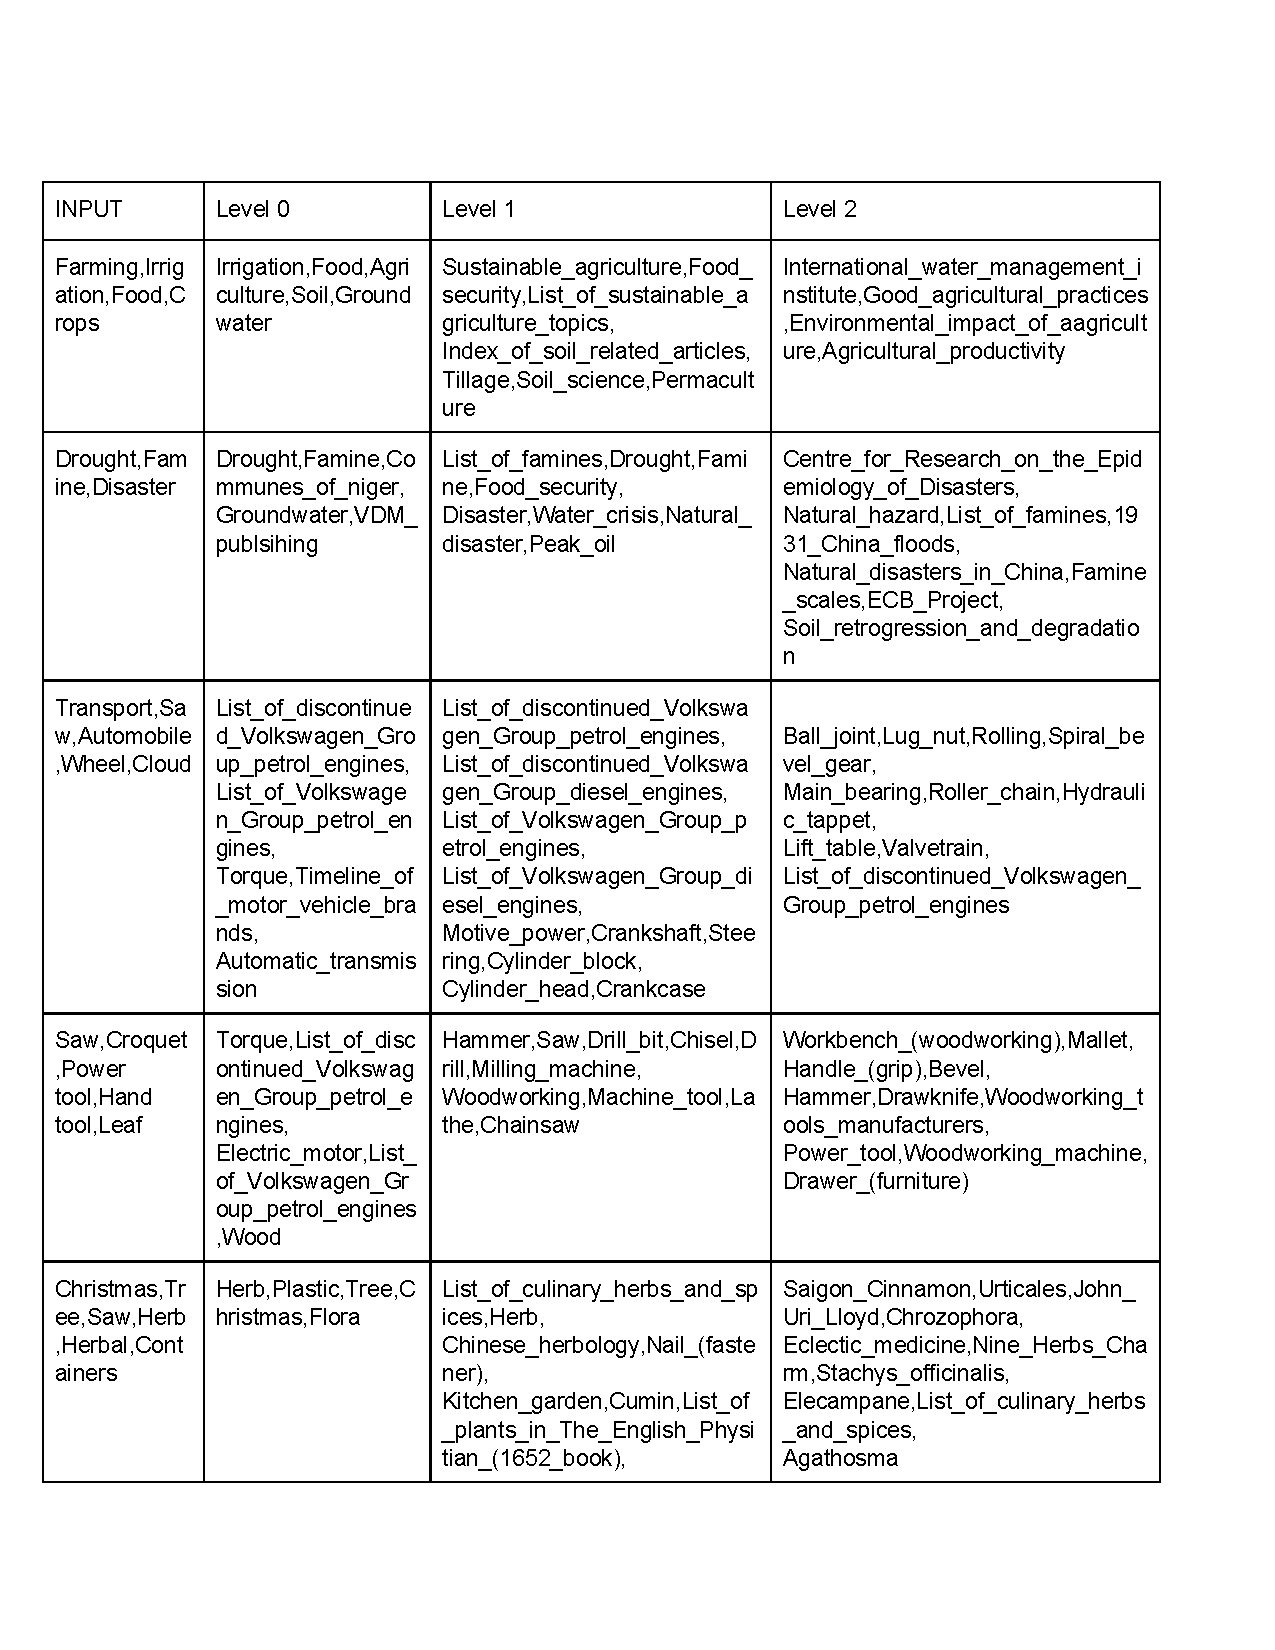
\includegraphics{file.pdf}
\end{figure}

\subsubsection{Corpora end point}
This allows users to upload their own set of documents into concept insights service. The provided documents are annotated and indexed by the service automatically. The query methods of this end point allows users to access the index created and analysis regarding the documents.\\

The following table gives the sample input and outputs for related\_concepts function for various values of level parameter.

\newpage
\section{Implementation Done}

\subsection{Reducing Latency By Disabling AutoSuggestions} 
Previously in the game, when the user enters a tag, auto suggestions are shown and he/she has to wait until the suggestions are shown and then select the appropriate tag for the video. Now, this latency is reduced by disabling auto sugegstions featute and after the user completes entering a tag, he/she has to press enter. Then automatically the word is mapped to its first suggestion and score is assigned to that tag on the fly.

\subsubsection{Advantages}
\begin{itemize}
\item User need not wait for the sugegstions to be shown
\item He/she can completely concentrate on providing tags, rather than changing the tag until suggestions are shown
\end{itemize}

\subsubsection{Disadvantages} 
\begin{itemize}
\item Sometimes the first suggestion may not be the appropriate one with reference to the video.\

For example, if the user enters the tag "social", the first suggestion it gets mapped to is the word "facebook", which may not always be the appropraite tag for given video.\

This problem has to be solved by mapping the user entered tag to the most meaningful suggestion(semantically) rather than the first suggestion.
\end{itemize}

\subsection{SpellCheck using Mashape\cite{i1}}

\textbf{Mashape\cite{i1} } is an open source webspell checker service that provides suggestions for spelling corrections for specified text.

Previously in the game, while entering a tag, user had choosen from one of the suggestions shown by concept insights service. So there is no need of spell checker.
But now, as the auto suggestion feature is disabled there may be possibility that the user misspells a word and hence the necessity of correcting it arises. If we do not correct the misspelled word, it cannot be mapped to any word in the concept insights service corpus and hence this tag cannot be shown in Leaderboard.    



\subsection{Suggesting tags}
Based on the tags the player had entered, and using \textbf{related\_concepts} function of concept insights service of IBM Watson some additional tags are suggested.
  

\newpage
\subsection{User stories}
\subsubsection{User story for entire tagVideo game}



\begin{figure}[h]
\begin{center}
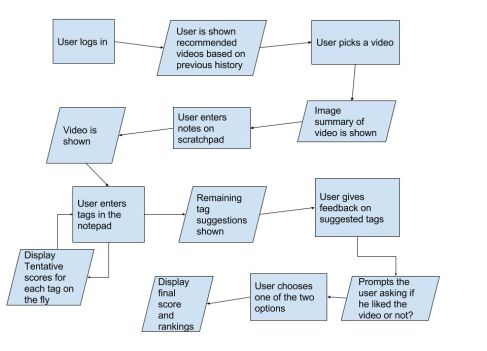
\includegraphics{images/userstory2_mod.jpg}
\caption{User story for entire tagVideo game}
\label{User story for entire tagVideo game}
\end{center}
\end{figure}

\newpage
\subsubsection{User story for entering tags}



\begin{figure}[h]
\begin{center}
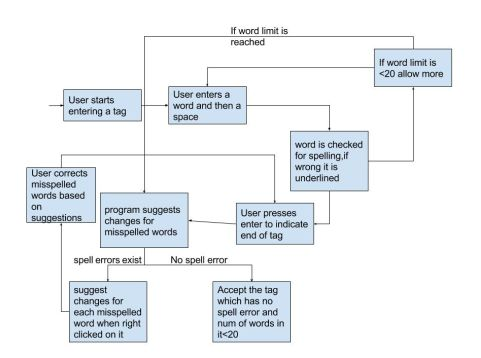
\includegraphics{images/userstory1_mod.jpg}
\caption{User story for entering tags}
\label{User story for entering tags}
\end{center}
\end{figure}




\newpage
\section{Conclusion}
 The first step in optimizing game is to remove restriction on user to enter only concepts given by concept insights service .In this process, we reduced the latency by removing auto suggestions and making user enter his own rich set of tags.When user enters his own tags, there might be possibility of spell erros and hence spell check has been integrated.

\newpage
\section{Future Scope}
\subsection{Major Challenges to Overcome}
\paragraph{} Removing the dependency on IBM Watson corpus and building our own domain specific knowledge graph of categories.
\subsection{Work in stage 2}
The following major tasks are planned to be done in stage 2:
\begin{itemize}
\item Recommend videos to the user based on the viewing history.
	\item Flashing of the image summary of the video, before the user sees the entire video
	\item Implementation of asking user's feedback on tags entered by other playes, at the end of viewing the video.
	
	
\end{itemize}








\newpage
\section*{Acknowledgements}
I would like to thank my guide, Prof. Ganesh Ramakrishnan for the consistent directions he has fed into my work.

\newpage
\pagestyle{empty}
\bibliographystyle{amsplain}
\nocite{*}
%\bibliography{database}



\begin{thebibliography}{9}
\bibitem{esp}
  Luis von Ahn and Laura Dabbish.
    \textit{ Labeling Images with a Computer Game.}
Proceeding
CHI '04 Proceedings of the SIGCHI Conference on Human Factors in Computing Systems
Pages 319-326 



\bibitem{conceptinsights}
https://watson-api-explorer.mybluemix.net/swagger.html?url=/listings/concept-insights-v2.json , [Online; accessed 08-October-2015].


\bibitem{i1} 
https://market.mashape.com/montanaflynn/spellcheck,      [Online; accessed 02-October-2015].

  
\end{thebibliography}
 
\end{document}

\end{document}
